\chapter{Results and Discussion}

\section{Camera Network}
Camera Network provided a great asset in acquiring the relevant dataset. The system is aimed at real-time processing of multiple camera feed. However, minor steps backs are faced during the footage capture. The NVR firmware is maintained by a Chinese video surveillance manufacturer, Uniview, abbreviated as UNV. The software interface have lower support for live streaming of footage, which leads to complex method of acquiring frame. The NVR also didn't expose API for streaming or playback of recorded footage. The camera occasionally provides with corrupted frames (see figure \ref{fig:corrupted}), leading to false detection. Camera footage is extracted at 25 FPS, $1920*1080$ px.

% Blacklisting of currupted framed used 
% No streaming or playback api for recorded video

\begin{figure}[!ht]
	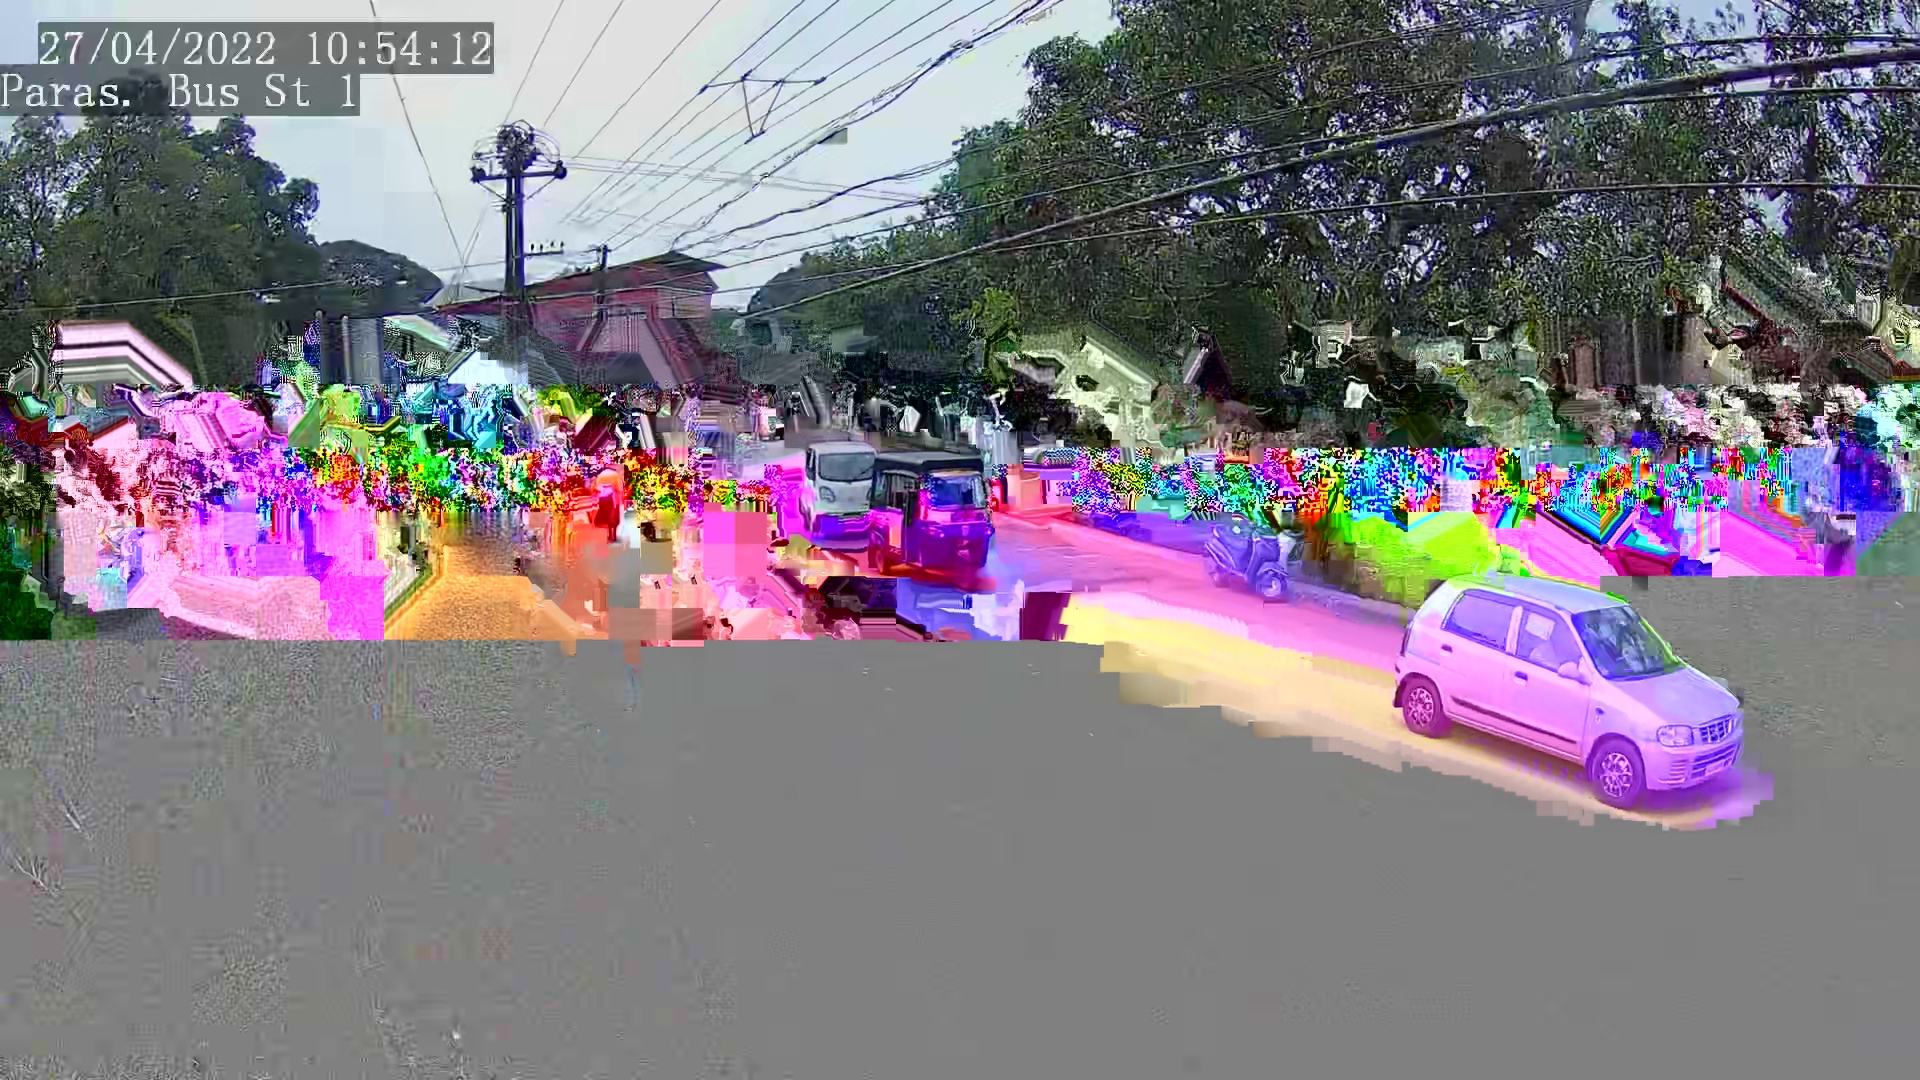
\includegraphics[width=0.32\linewidth]{Images/camera_footage/corrupted1} \hfill
	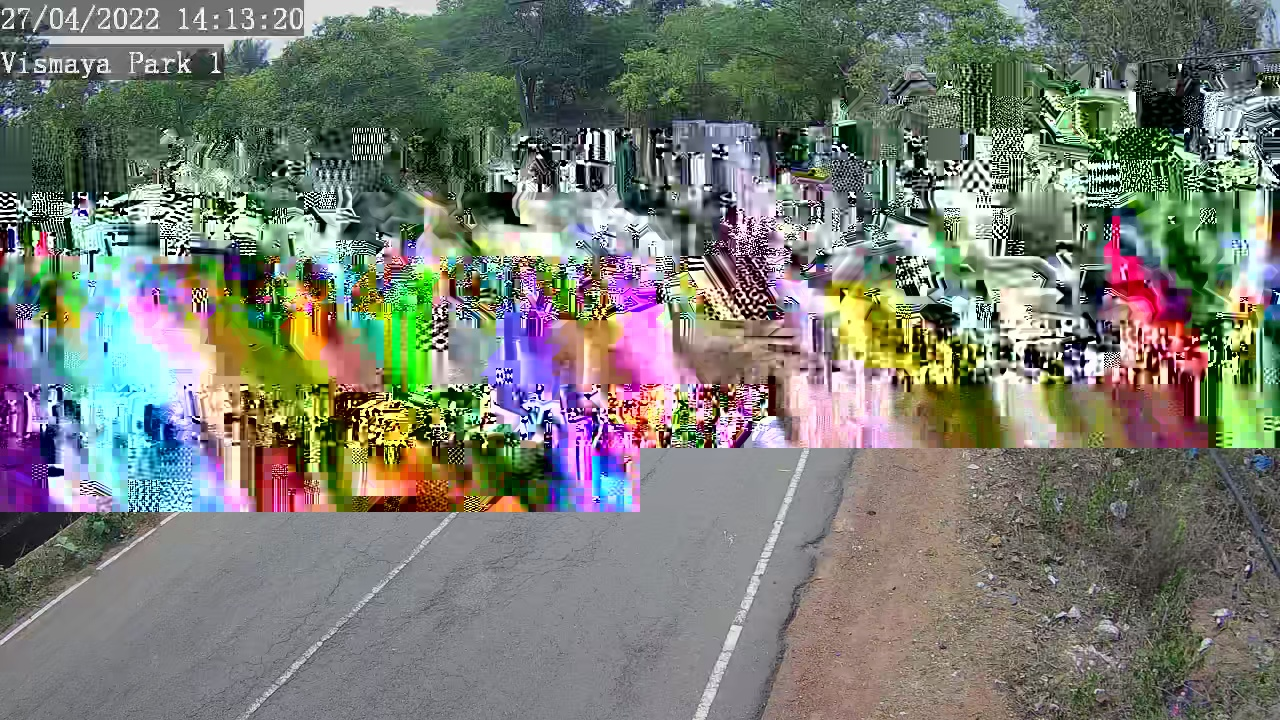
\includegraphics[width=0.32\linewidth]{Images/camera_footage/corrupted2} \hfill
	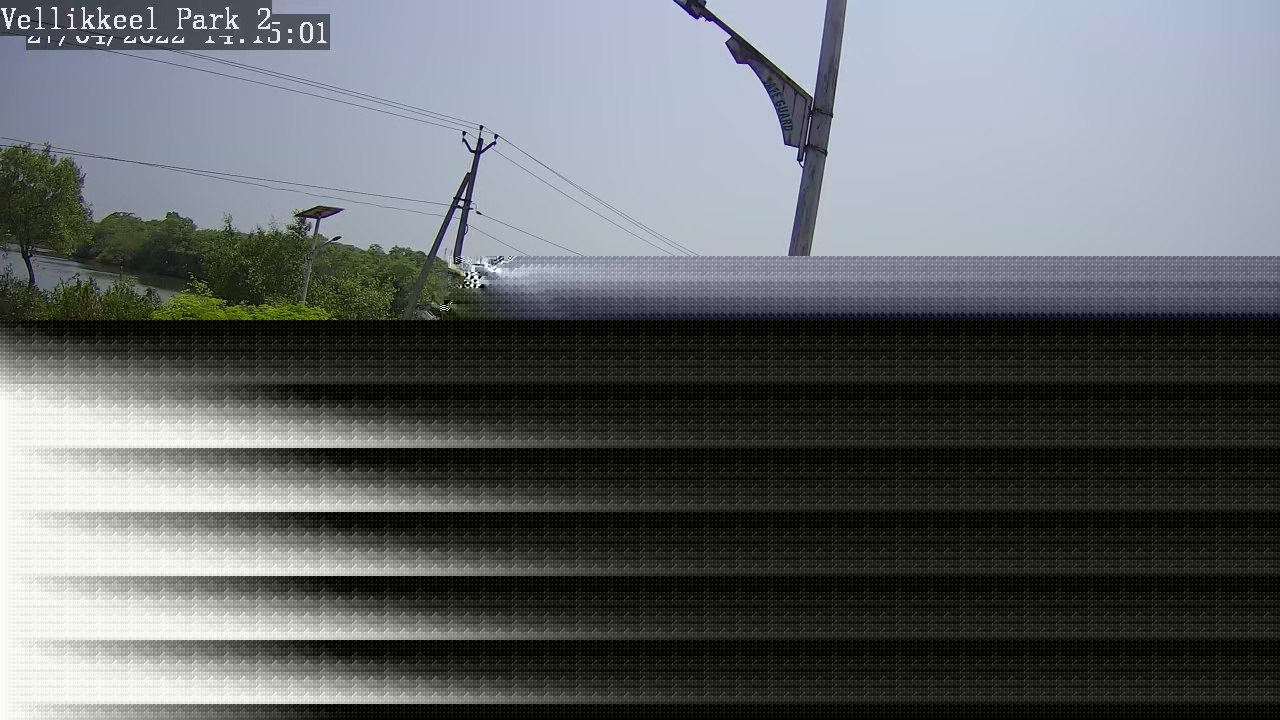
\includegraphics[width=0.32\linewidth]{Images/camera_footage/corrupted3} \\ 
	\\
	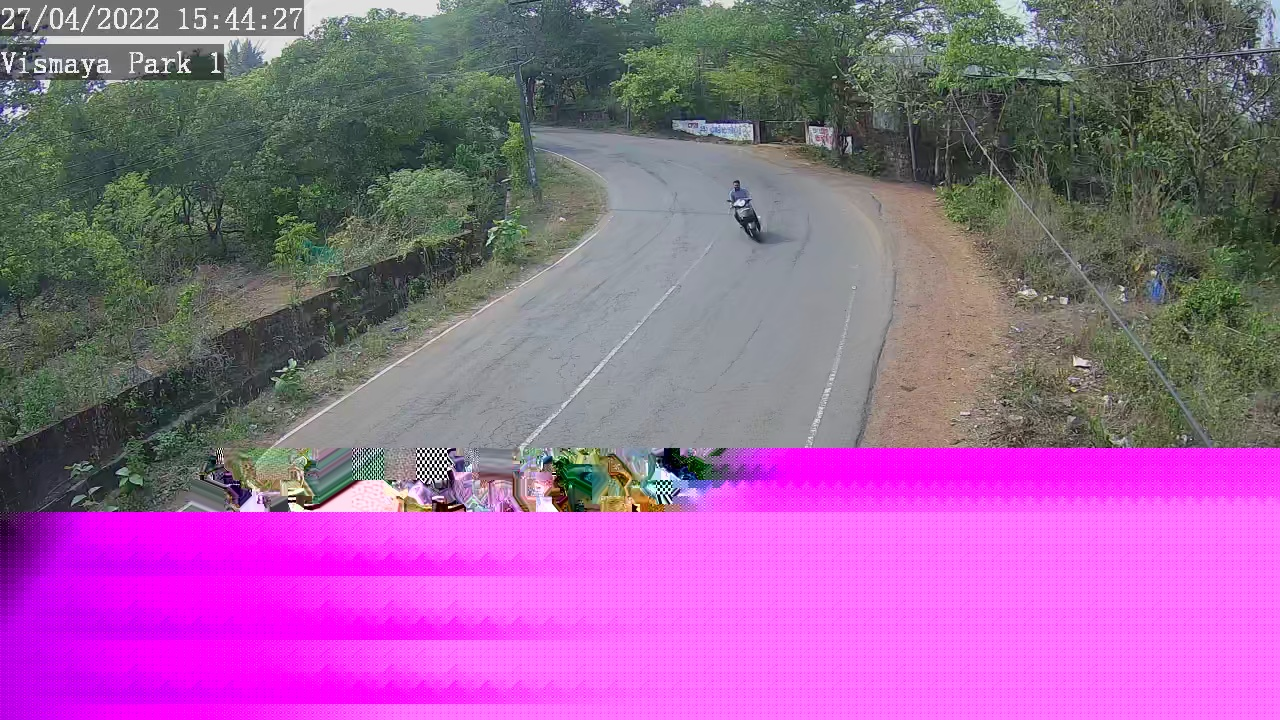
\includegraphics[width=0.32\linewidth]{Images/camera_footage/corrupted4} \hfill
	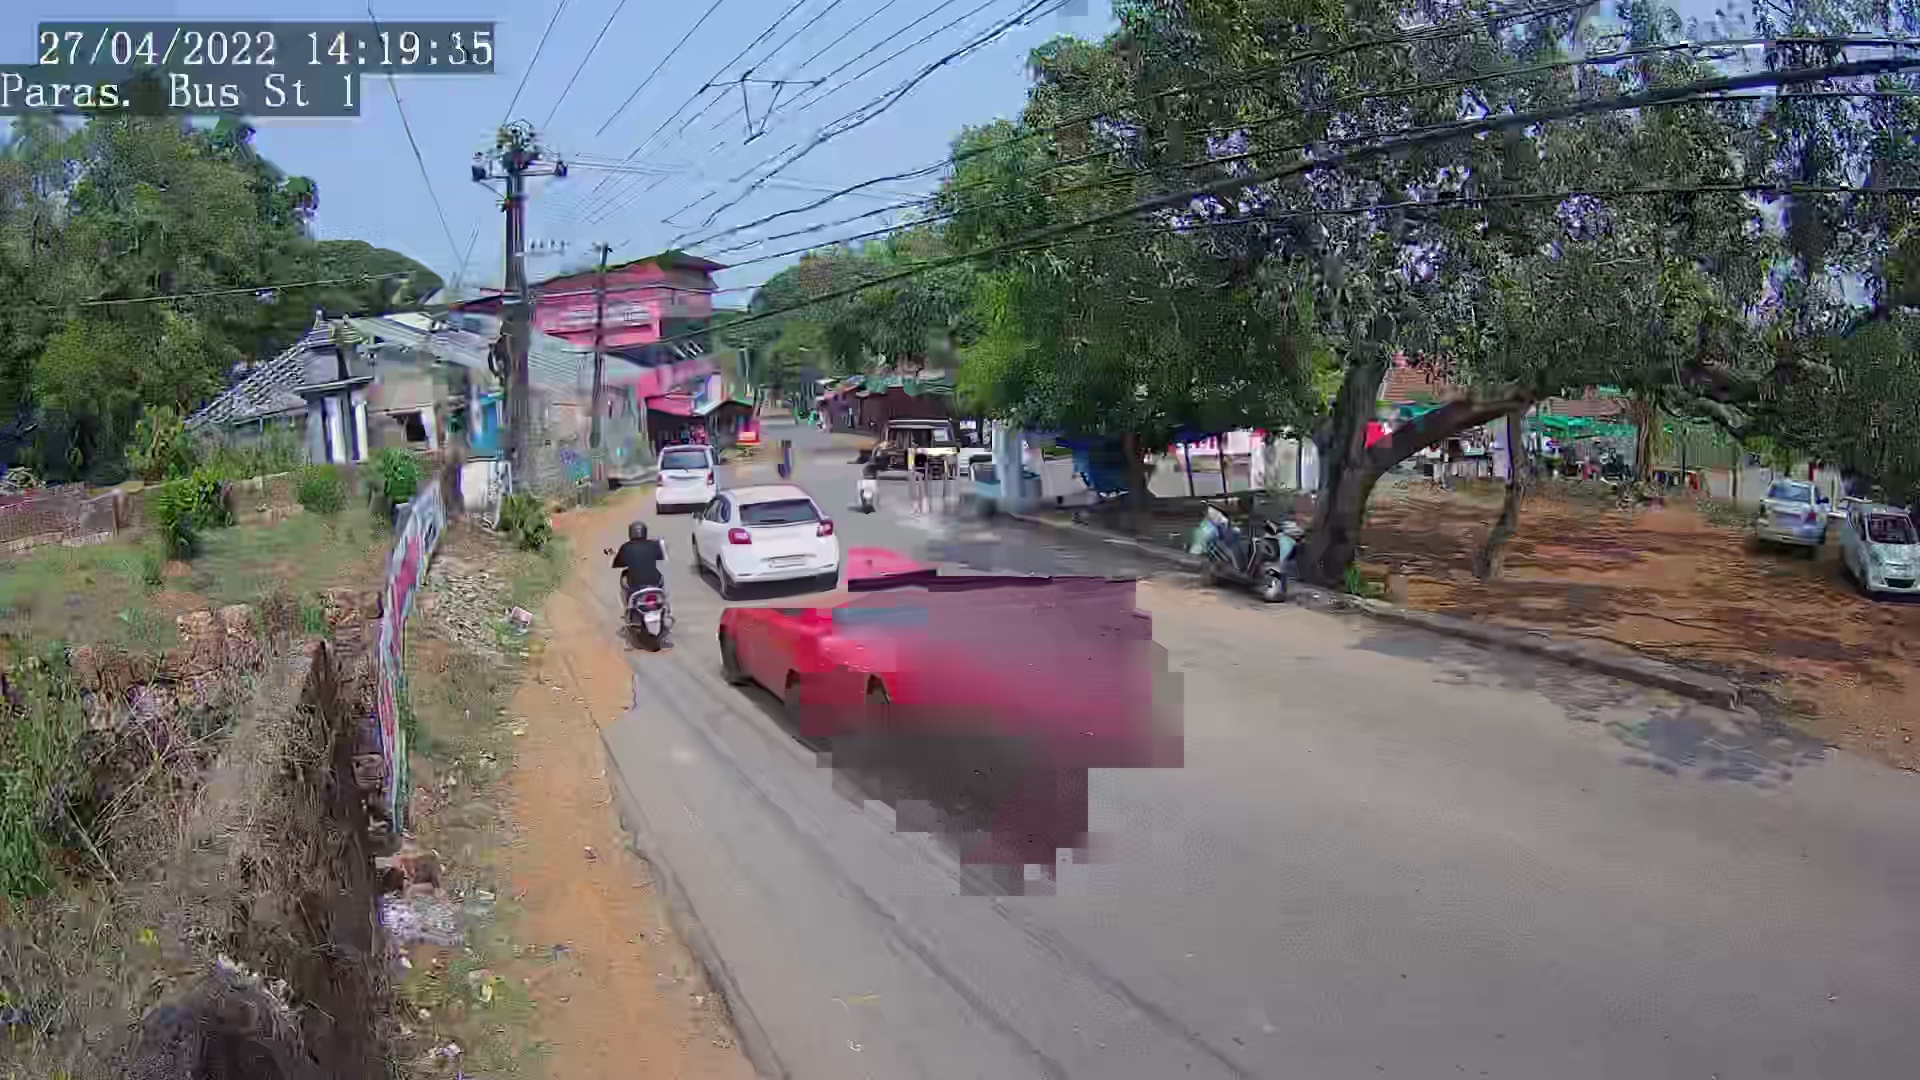
\includegraphics[width=0.32\linewidth]{Images/camera_footage/corrupted5} \hfill
	
\includegraphics[width=0.32\linewidth]{Images/camera_footage/corrupted6} 
	\caption{Corrupted Camera footage}
	\label{fig:corrupted}
\end{figure}

\section{YOLOv4}
YOLOv4 model is trained with 1559 images for 9 classes as illustrated in table \ref{tab:dataset_sum1}. Model accuracy is easily calculated by Darknet and is shown in table \ref{tab:yolo_matrix} and \ref{tag:yolo_score}. The model, in the deployment ran at slower speed of about 19.1 FPS. The decrease in speed is due to the unwanted processing of dead/corrupted frame. Speed can also be improved by reducing the yolo network size, compromising accuracy.

\begin{table}[!ht]
	\centering
	\begin{tabular}{|l|l|l|l|}
		\hline
		Class label    & True Positive & False Positive & Avg Precision \\ \hline
		auto           & 424           & 38             & 98.25\%       \\ \hline
		bus            & 327           & 42             & 99.57\%       \\ \hline
		tempo traveler & 76            & 7              & 97.12\%       \\ \hline
		tractor        & 130           & 2              & 98.44\%       \\ \hline
		truck          & 516           & 33             & 99.28\%       \\ \hline
		van            & 227           & 22             & 98.14\%       \\ \hline
		two wheeler    & 770           & 241            & 91.62\%       \\ \hline
		car            & 644           & 91             & 96.99\%       \\ \hline
		jcb            & 0             & 0              & 100.00\%      \\ \hline
	\end{tabular}
	\caption{YOLOv4 accuracy matrix}
	\label{tab:yolo_matrix}
\end{table}

\begin{table}[!ht]
	\centering
	\begin{tabular}{|l|l|}
		\hline
		Precision            & 87\%    \\ \hline
		Recall               & 96\%    \\ \hline
		F1-score             & 91\%    \\ \hline
		True Positive        & 3114    \\ \hline
		False Positive       & 476     \\ \hline
		False Negative       & 134     \\ \hline
		Avg IoU              & 72.13\% \\ \hline
		Mean Avg precision   & 97.71\% \\ \hline
		Total Detection Time & 1166 Seconds \\ \hline
		Detection count      & 12349 \\ \hline
		Unique truth count   & 3257 \\ \hline
	\end{tabular}
	\caption{YOLOv4 evaluation}
	\label{tag:yolo_score}
\end{table}

\begin{figure}[ht!]
	\centering
	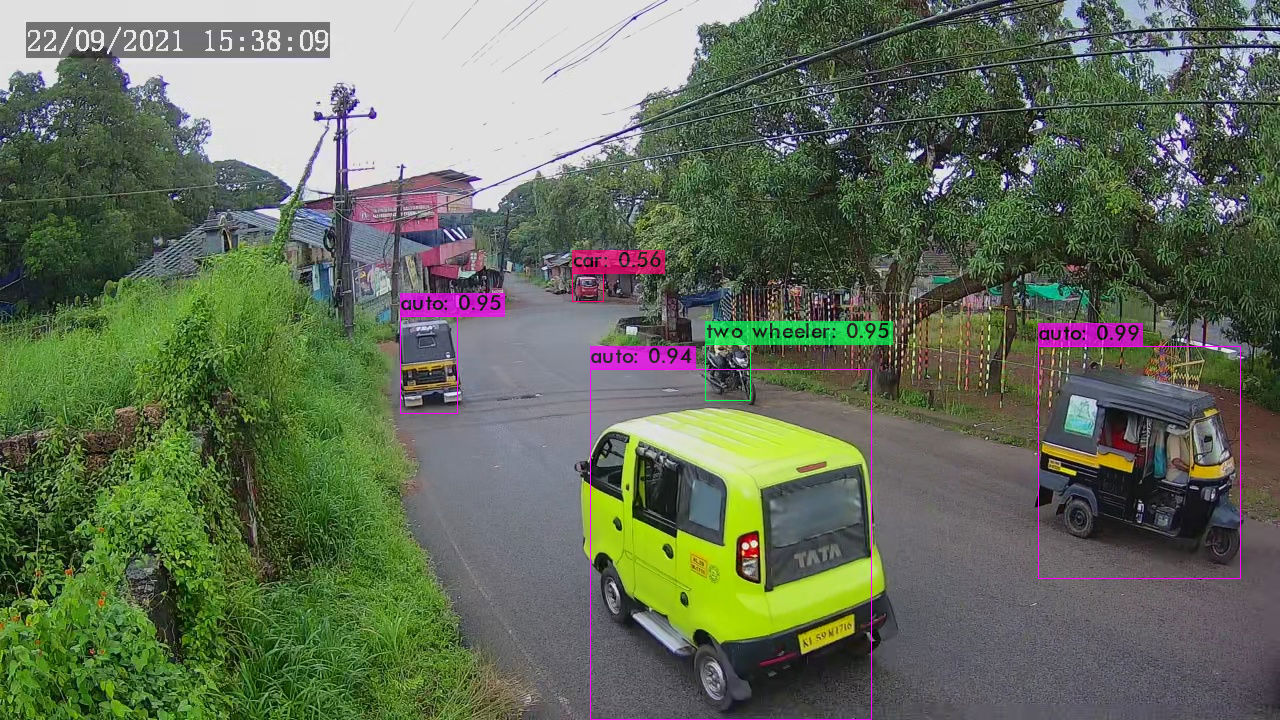
\includegraphics[width=0.8\linewidth]{Images/predictions}
	\caption{YOLOv4 vehicle predictions}
\end{figure}


\section{DeepSORT}
Ground Truth dataset was not available to quantize the result. However, via visual inception, it was found that the model was able to assign correct ID number to most of the vehicles. It was observed that such an increase in accuracy was observed due to the presence of Kalman filtering algorithm. The deep matrix association for humans was trigger only at the presence of humans. It lead to a mismatch where traditional Kalman filter tries to re-Id the bounding boxes, where as deepSORT tries to match human description leading to wrong answer. The anomaly can be strongly seen in public transport bus. Building of deep matrix for vehicle can improve the system.

\section{Siamese Network}
Proper Siamese Network was unable to construct, as the layers of yolov4 models was not able to selectively extract. The YOLOV4 model have tight coupling between layers, with multiple output and input vectors. The model is originally implement in Darknet.  This provided hindrance during the extraction of layers using keras and python.

\section{Other Limitations}
\begin{itemize}
	\item Current detection rate is about 19.1 FPS, which is not ideal to process multiple camera footage concurrently in real-time.
	\item The model was not trained to extract color class labels. Use of K-means gives poor realization of vehicle color. Background colors are also being extracted in K-means.
	\item User needs to visually inspect the similarity of target vehicle across the network, Siamese network is not completely realized.
	\item Limited user parameters for vehicle description. All parameter needs to be provided for search to begin.
	\item Heavy system resource utilization. Parsing larger network require higher RAM and CPU utilization. Larger volume of footage needs to be processed and stored.
	\item GPU with Nvidia MPS enabled or support for GPU partitioning was not available. So even simple model running in CUDA allocates whole GPU memory. About 5GB of GPU is being completely reserved and locked by YOLO model. 
	\item No Multi-GPU systems to fully utilize multiple parallel instance of AI Engine in same server.
	\item On the fly transcoding was needed to convert HEVC RTSP stream to RTMP stream for Nginx Media Server, consuming significant resources.
	% GPU not enabled with Nvidia MPS
	% No MultiGPU system available
	\item Sharing streaming key to all users, can cause breach of security and unauthorized users may access 
	\item Not sharing streaming key would result in multiple FFmpeg instances transcoding same footage.
	
\end{itemize}



